\documentclass[a4paper,titlepage]{report}
\usepackage{graphicx}
\usepackage[a4paper, margin=1in]{geometry}
\usepackage{titlesec}
\usepackage[dvipsnames]{xcolor}
\usepackage{amsmath}
\usepackage{booktabs}
\usepackage{cellspace}
\usepackage{tabularx}
\usepackage{caption}
\usepackage{calc}

\setlength\cellspacetoplimit{5pt}
\setlength\cellspacebottomlimit{4pt}

\definecolor{myBlue}{rgb}{0.0745, 0.2157, 0.4118}
\definecolor{myLightBlue}{rgb}{0, 0.5647, 0.5843}

\titleformat{\section}[hang]{\Large\bfseries\color{myBlue}}{}{0px}{}[\titlerule]
\titleformat{\subsection}[hang]{\large\bfseries\color{myLightBlue}}{}{0em}{}
\titleformat{\subsubsection}[hang]{\bfseries\color{myBlue}}{}{0em}{}

% Set the dimension of titles of chapters to \LARGE and 
\titleformat{\chapter}[display]
  {\normalfont\Large\bfseries}{}{0pt}{\LARGE}

% remove the word "Chapter" and the number from the title
\renewcommand{\chaptername}{}

\setcounter{tocdepth}{1} % Include only chapter and section in the table of contents

\begin{document}

\begin{titlepage}
    \centering
    \vspace*{\fill}
    {\LARGE \textbf{University of Pisa}}\\[0.5cm]
    {\Large \textit{Artificial Intelligence and Data Engineering}}\\[1.5cm]
    {\LARGE \textbf{Distributed Systems and Middleware Technologies}}\\[1cm]
    {\Large \textit{FLconsole documentation}}\\[10cm]
    {\large \textbf{Authors: Çolak F. Messina F. Nocella F.}}\\[0.5cm]
    {\large Academic Year 2023/2024}
    \vspace*{\fill}
\end{titlepage}


\tableofcontents

\chapter{Introduction and Project Overview}\label{ch:introduction-and-project-overview}


\section{Context and Project Objective}\label{sec:context-and-project-objective}

In this section, the context and objective of the project are described.

\section{Application Highlights}\label{sec:application-highlights}

In this section, the highlights of the application are presented.

\chapter{Analysis}\label{ch:analysis}


\section{Requirements}\label{sec:requirements}

In this section, the requirements of the project are presented.

\subsection{Functional Requirements}\label{subsec:functional-requirements}

The functional requirements of the project are described in this subsection.

\subsection{Non-Functional Requirements}\label{subsec:non-functional-requirements}

The non-functional requirements of the project are described in this subsection.

\subsection{Constraints/Other Requirements}\label{subsec:constraints/other-requirements}

Any constraints or other requirements on the project are described in this subsection.

\section{Actors}\label{sec:actors}

The actors who can interact with the web console system consist of the following:
\begin{itemize}
    \item \textbf{User:} The user is the actor who can browse the system to view running and completed experiments and their results.
    \item \textbf{Admin:} The admin is the actor who can manage the system, including creating and deleting configurations and experiments, and viewing the results of experiments.
\end{itemize}

\section{Use Case Modeling}\label{sec:use-case-modeling}

\subsection{Use Case Diagram}\label{subsec:use-case-diagram}

\begin{figure}[ht!]
    \centering
    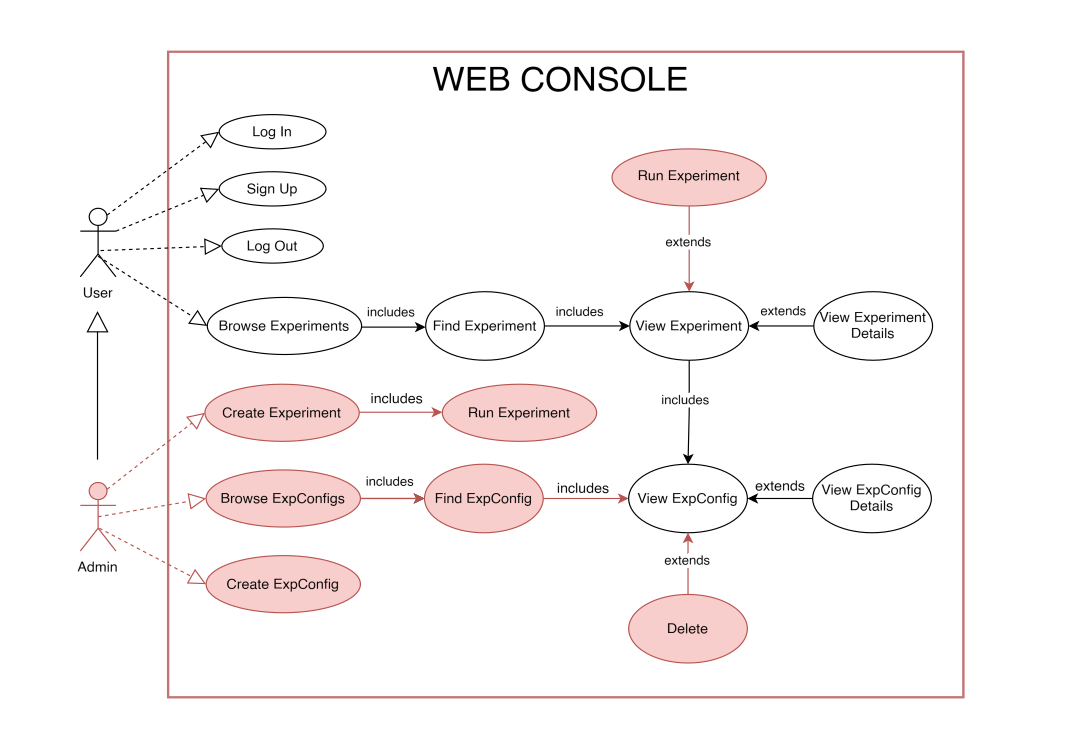
\includegraphics[width=0.8\textwidth]{images/2_analisys/FL_class_diag.drawio}
    \caption{Use Case Diagram}
    \label{fig:figure}
\end{figure}

\subsection{Scenarios}\label{subsec:scenarios}

\begin{table}[ht!]
    \centering
    \caption{Use Case: Find Recipes}
    \begin{tabular}{|Sl|Sl|}
        \hline
        \textbf{\textit{Use Case}}      & \textbf{Find Recipes}                            \\ \hline
        \textbf{Primary Actor}          & User                                            \\ \hline
        \textbf{Secondary Actor}         & -                                               \\ \hline
        \textbf{Description}             & Allows the user to find a specific recipe       \\ \hline
        \textbf{Pre-Conditions}          & User must be logged i                        \\ \hline
        \textbf{Main event steps}        & 1) The user navigates to the “Search” feature   \\
                                          & 2) The user enters a string                     \\
                                          & 3) The system searches the recipe database for  \\
                                          & matching results (title, keywords, description) \\ 
                                          & 4) Upon finding matching posts, the system      \\
                                         & displays the search results                     \\ \hline
        \textbf{Post-Conditions}         & The user views a list of recipes matching the   \\ 
                                         & search criteria if there are any                \\ \hline
        \textbf{Correlated Use cases}    & View Recipe, Browse Recipes                     \\ \hline
        \textbf{Alternative event steps} & -                                               \\ \hline
    \end{tabular}\label{tab:table}
\end{table}
\subsection{Analysis Class Diagram}\label{subsec:analysis-class-diagram}

The analysis class diagram of the project is presented in this subsection.

\subsection{Sequence Diagrams}\label{subsec:sequence-diagrams}

The sequence diagrams of the project are presented in this subsection.


\chapter{Design}

\section{Introduction}
This chapter aims to provide a detailed overview of the software architecture and database design of the project. It is essential for understanding the organization and structure of the system, as well as the design choices made to ensure the efficiency, scalability, and robustness of the software.

The design of the software architecture focuses on the organization and distribution of software components, defining roles, responsibilities, and interactions among them. Key architectural decisions guiding the project's development will be presented within this context.

Additionally, the database design will be examined, with particular attention to the decision to use a NoSQL database like MongoDB. This decision was motivated by the need to adapt to the specific requirements of the project, including flexible management of unstructured data and horizontal scalability.


\section{Software Architecture}

\begin{figure}[ht!]
    \centering
    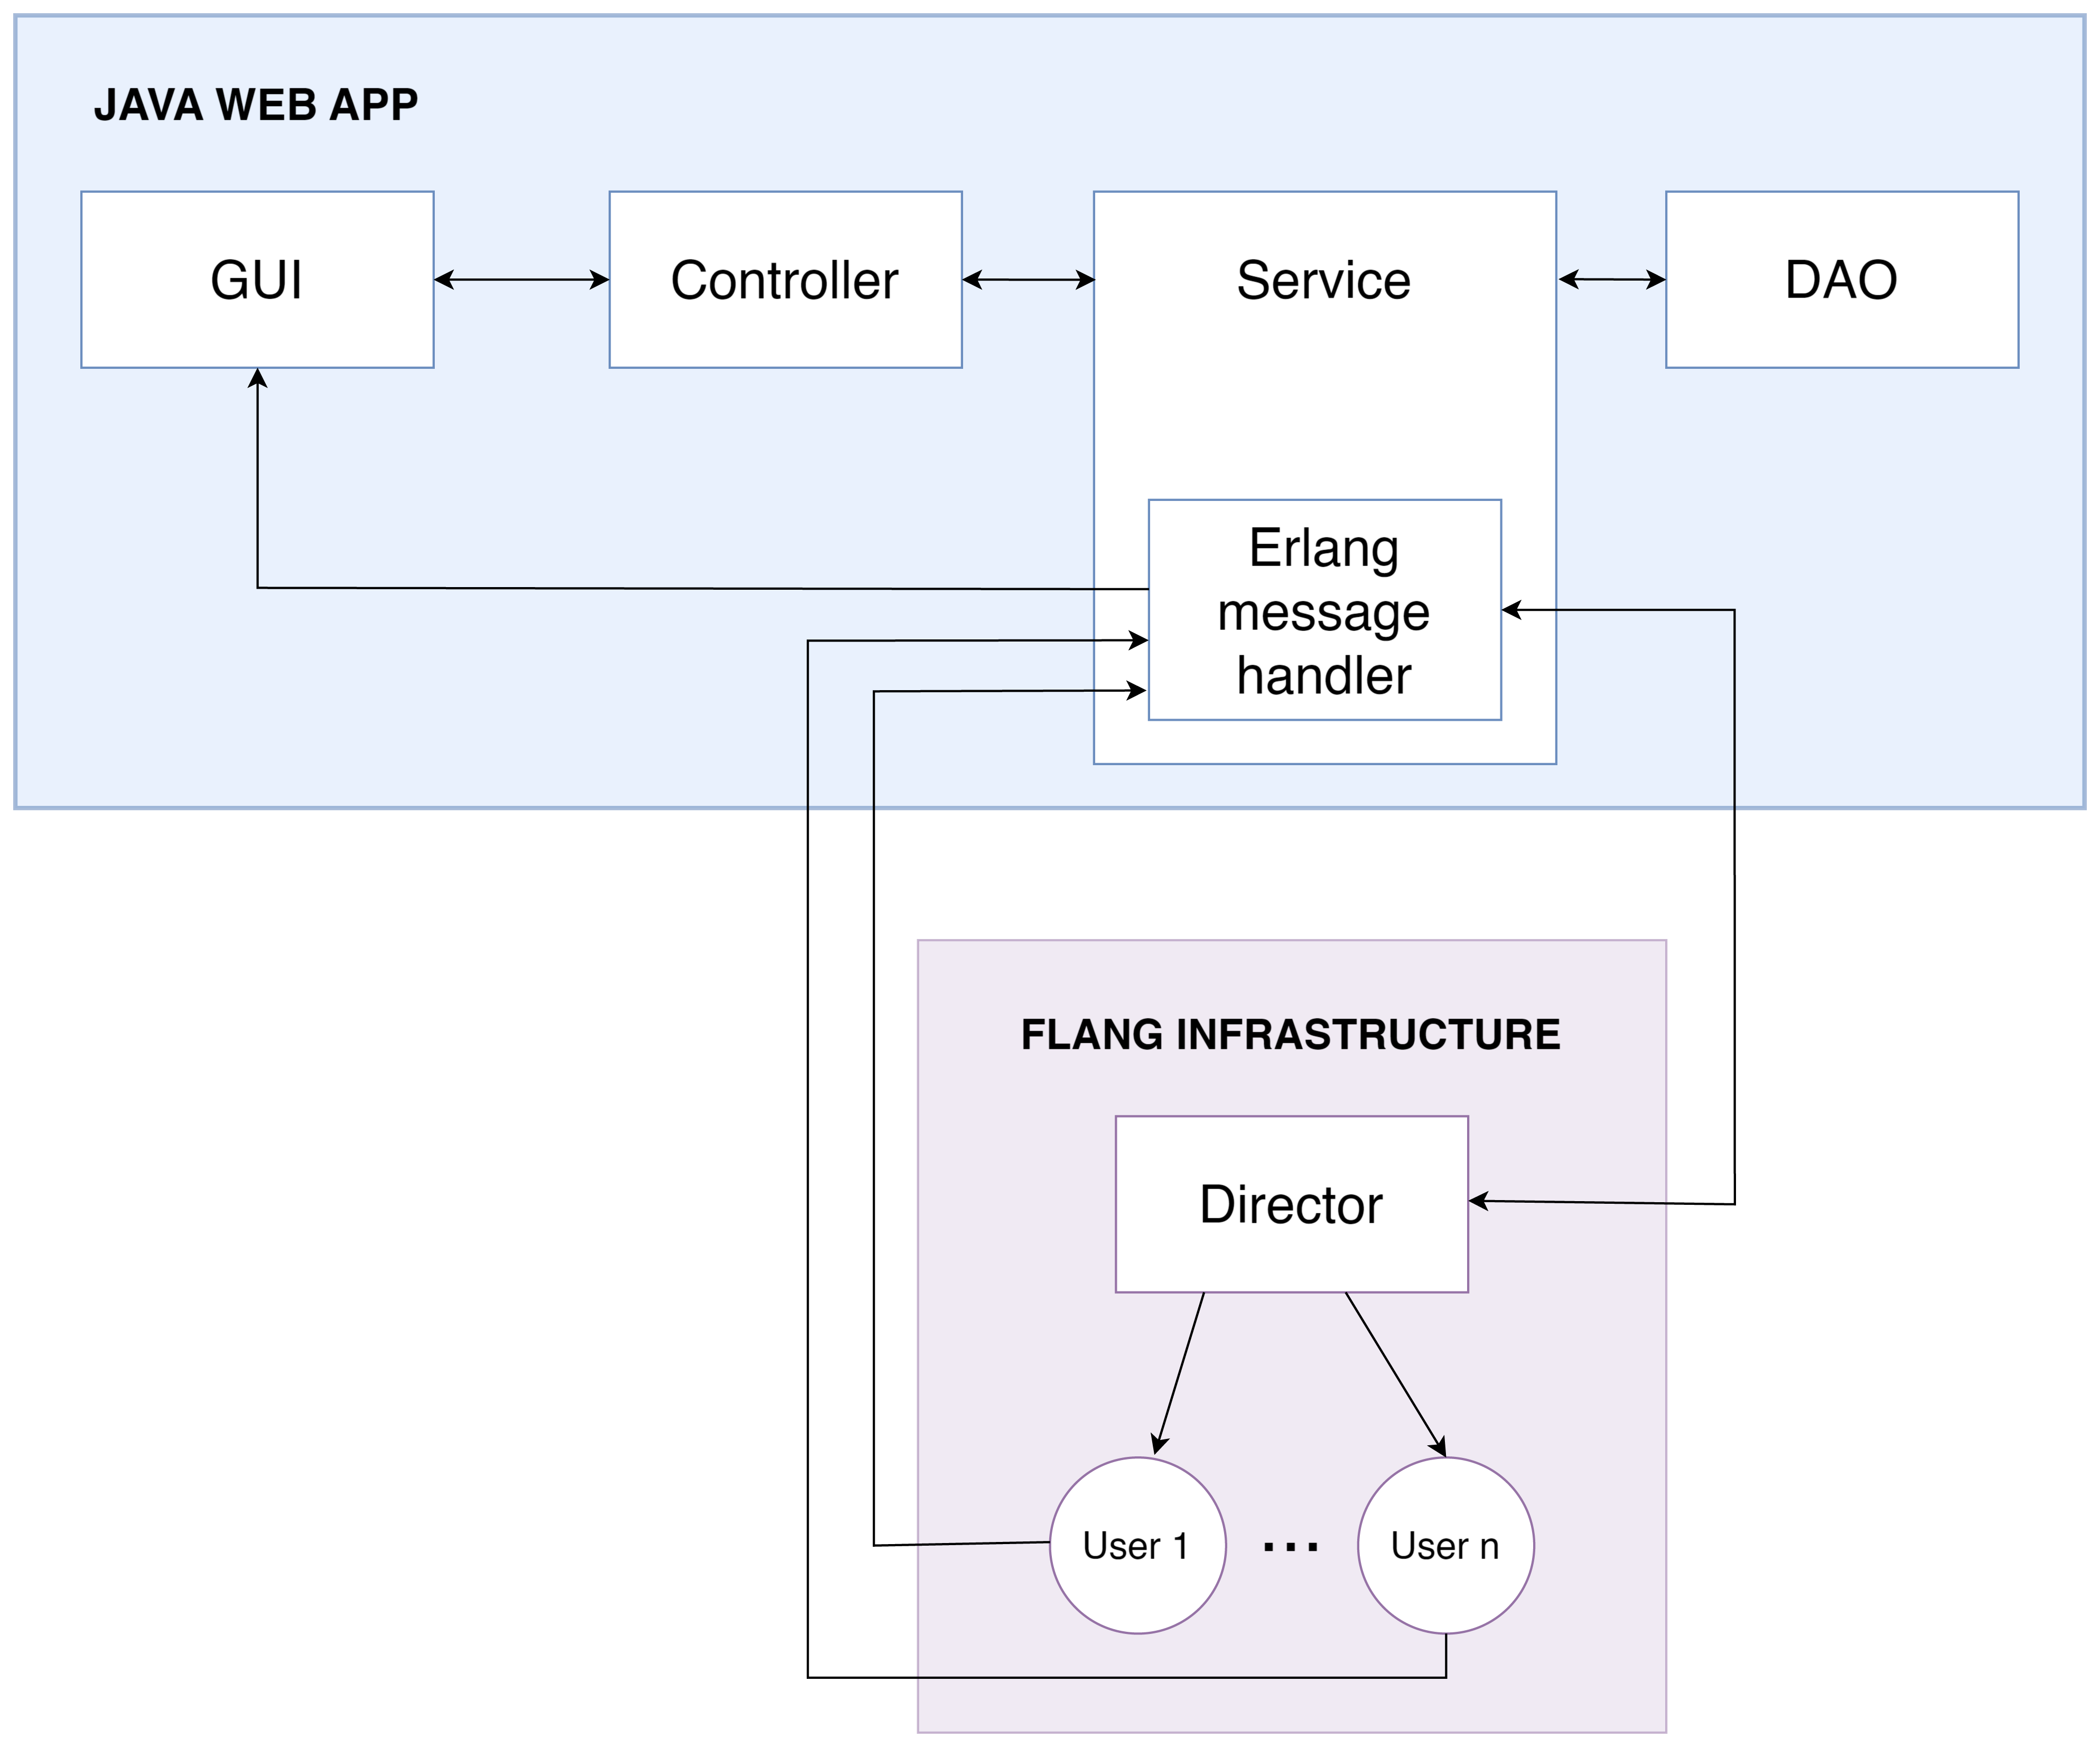
\includegraphics[width=0.8\textwidth]{images/2_analisys/FL_proj_Arch_FINAL.png}
    \caption{System Architecture}
    \label{fig:system_architecture}
\end{figure}


\newpage
\section{Database Design}

\subsection{MongoDB}
\subsubsection{Collections}
\textbf{ExpConfig document example:} \begin{verbatim}
        {
            "_id": {
              "$oid": "6613f8b7aed2e52b006dea10"
            },
            "name": "TestConfig",
            "algorithm": "fcmeans",
            "codeLanguage": "python",
            "clientSelectionStrategy": "probability",
            "clientSelectionRatio": 1,
            "minNumberClients": 2,
            "stopCondition": "max_number_rounds",
            "stopConditionThreshold": 5,
            "maxNumberOfRounds": 10,
            "parameters": {
              "targetFeature": "16",
              "lambdaFactor": "2",
              "numFeatures": "16",
              "seed": "10",
              "numClusters": "10"
            },
            "creationDate": {
              "$date": "2024-04-08T14:01:27.232Z"
            },
          }
    \end{verbatim}
\textbf{Experiment document example:} \begin{verbatim}
        {
            "_id": {
              "$oid": "661c3d780bb4be3bd9b891b9"
            },
            "name": "ExpTest",
            "expConfig": {
              "_id": {
                "$oid": "6613f8b7aed2e52b006dea10"
              },
              "name": "TestConfig",
              "algorithm": "fcmeans"
            },
            "creationDate": {
              "$date": "2024-04-14T20:32:56.022Z"
            },
            "status": "FINISHED",
            "flExpId": "\"d9d1bc7c-d733-4219-b4fb-16a3849db323\"",
            "modelPath": "\\FL_models\\exp_661c3d780bb4be3bd9b891b9.bin"
          }

    \end{verbatim}

\newpage
\textbf{ExperimentMetrics document example:} \begin{verbatim}
        {
            "_id": {
              "$oid": "66144b5337a2fd7f67582f67"
            },
            "expId": "661c3d780bb4be3bd9b891b9",
            "type": "STRATEGY_SERVER_METRICS",
            "hostMetrics": {
              "cpuUsagePercentage": 5,
              "memoryUsagePercentage": 9.27
            },
            "modelMetrics": {
              "FRO": 845.7339394664009
            },
            "timestamp": {
              "$date": "1970-01-20T19:43:26.034Z"
            },
            "round": 1,
          }
    \end{verbatim}

\textbf{User document example:} \begin{verbatim}
    {
        "_id": {
          "$oid": "6611252030f96a50aebda458"
        },
        "email": "admin@example.com",
        "password": "P@ssw0rd",
        "creationDate": {
          "$date": "2024-04-06T10:34:08.669Z"
        },
        "role": "admin",
        "configurations": [
          "6613f8b7aed2e52b006dea10"
        ],
        "experiments": [{
            "_id": {
              "$oid": "661c3e800bb4be3bd9b891da"
            },
            "name": "ExpTest",
            "config": "TestConfig",
            "creationDate": {
              "$date": "2024-04-14T20:32:56.022Z"
            }
          }]
      }

    \end{verbatim}
\newpage
\section{Message Handler}

\subsection{Erlang for Message Passing}
The message handler is implemented using the Erlang programming language. Erlang is a functional programming language designed for building scalable and fault-tolerant systems. It is particularly well-suited for building distributed systems, thanks to its lightweight processes and built-in support for message passing. In this project, it's utilized the Jinterface library, which allows to write Java code that can communicate with Erlang processes to send and receive messages, arriving from the FLang Infrastructure and vice versa.

\subsection{Message Structure}
\begin{itemize}
    \item Experiment Queued:
          \begin{verbatim}
        {
            "type": "experiment_queued",
            "timestamp": "1712206255"
        }
    \end{verbatim}

    \item Worker Ready:
          \begin{verbatim}
        {
            "type": "worker_ready",
            "timestamp": "1712206257",
            "client_id": "1"
        }
    \end{verbatim}

    \item Strategy Server Ready:
          \begin{verbatim}
        {
            "type": "strategy_server_ready",
            "timestamp": "1712206257"
        }
    \end{verbatim}

    \item All Workers Ready:
          \begin{verbatim}
        {
            "type": "all_workers_ready",
            "timestamp": "1712206257"
        }
    \end{verbatim}

    \item Start Round:
    \begin{verbatim}
      {
          "type": "start_round",
          "timestamp": "1712206257",
          "round": "1"
      }
    \end{verbatim}
    
     \newpage

    \item End Round:
      \begin{verbatim}
      {
        "type": "end_round",
        "timestamp": "1712206260",
        "round": "1"
      }
    \end{verbatim}

    \item Strategy Server Metrics:
      \begin{verbatim}
      {
        "type": "strategy_server_metrics",
        "timestamp": "1712206264",
        "round": "2",
        "hostMetrics": {
          "cpuUsagePercentage":39.4,
          "memoryUsagePercentage": 52.69
        }
         "modelMetrics":{
          "FRO":"0.13237183370436725"
        }
      }
    \end{verbatim}
\end{itemize}

\subsection{Description of the Erlang Message Handler Module}
The Erlang message handler module is a crucial component of the system responsible for managing incoming messages, processing them accordingly, and facilitating communication between different parts of the distributed system. It encapsulates the logic for handling various types of messages, such as error notifications, stop signals, and data updates, ensuring proper routing and processing. Additionally, the module provides interfaces for sending and receiving messages, abstracting the underlying communication mechanisms and enabling seamless integration with other system components. Its robust design and fault-tolerant features contribute to the overall reliability and performance of the distributed system.
\chapter{Implementation}

\section{Development Environment}

The development environment used for the project is described in this section.

\section{Main Modules}

The main modules of the project are described in this section.

\section{Configuration}

The configuration of the project is described in this section.

\section{Data Access}

The data access layer of the project is described in this section.

\section{Data Transfer}

The data transfer mechanisms used in the project are described in this section.

\section{Service}

The services provided by the project are described in this section.

\section{User Interface}

The user interface of the project is described in this section.

\section{Adopted Patterns and Techniques}

The patterns and techniques adopted in the project are described in this section.

\chapter{Testing}

\section{Structural Testing}

The structural testing performed on the project is described in this section.

\subsection{JUnit Testing}

The JUnit testing performed on the project is described in this section.

\subsubsection{UserDAO}
\begin{figure}[ht!]
    \centering
    
\includegraphics[width=0.8\textwidth]{images/placeholder.jpg}
    \caption{User DAO tests}
    \label{fig:u_dao_test}
\end{figure}

\newpage
\subsubsection{ConfigurationDAO}
\begin{figure}[ht!]
    \centering
    
\includegraphics[width=0.8\textwidth]{images/placeholder.jpg}
    \caption{Configuration DAO tests}
    \label{fig:c_dao_test}
\end{figure}

\newpage
\subsubsection{ExperimentDAO}
\begin{figure}[ht!]
    \centering
    
\includegraphics[width=0.8\textwidth]{images/placeholder.jpg}
    \caption{Experiment DAO tests}
    \label{fig:e_dao_test}
\end{figure}

\newpage
\section{Functional Testing}

The functional testing performed on the project is described in this section.

\subsection{Test Cases}

\begin{table}[ht!]
    \centering
    \caption{Test case}
    \begin{tabularx}{\textwidth}{|Sl|S{X}|S{X}|S{X}|S{X}|S{X}|}
        \hline
        \textbf{Id} & \textbf{Description} & \textbf{Input} & \textbf{E. Output} & \textbf{Output} & \textbf{Outcome} \\ \hline
        U\_T\_01    & Lorem Ipsum          & Lorem Ipsum    & Lorem Ipsum         & Lorem Ipsum     & Lorem Ipsum      \\ \hline
        U\_T\_02    & Lorem Ipsum          & Lorem Ipsum    & Lorem Ipsum         & Lorem Ipsum     & Lorem Ipsum      \\ \hline
        U\_T\_03    & Lorem Ipsum          & Lorem Ipsum    & Lorem Ipsum         & Lorem Ipsum     & Lorem Ipsum      \\ \hline
        U\_T\_04    & Lorem Ipsum          & Lorem Ipsum    & Lorem Ipsum         & Lorem Ipsum     & Lorem Ipsum      \\ \hline
        U\_T\_05    & Lorem Ipsum          & Lorem Ipsum    & Lorem Ipsum         & Lorem Ipsum     & Lorem Ipsum      \\ \hline
    \end{tabularx}
\end{table}

\chapter{Conclusion}

%In this chapter, we summarize the key points of the document and discuss possible future directions for the project.

This chapter summarizes and highlights the key points of the document like architecture, implementation details, user interface components and
discusses possible future directions for the project of Federated Learning Web Console.


\subsection*{Key Points}
In this project Federated Learning Web Console is introduced which is a centralized platform for managing FL experiments with using Java and Erlang as primary programming languages,
Spring as a Java framework and MongoDB as a database. As a main project architectural structure, the project follows the MVC pattern. Various and functional models are implemented in
the project such as Configuration, Data Access Object, Services and User Interface with their specific roles and functionalities for serving the application. With the help of this
architecture FL Web Console project ensures a scalable design and having seamless functionality between different components. The user interface includes essential pages to provide
fully functional experience for the user. Those pages are login/signup, user/admin dashboard, profile page and experiment details.

\subsection*{Future Directions}
The project has a lot of potential for future improvements and enhancements. Some of the possible future directions are:
%???


\end{document}